\documentclass[12pt]{article}

% PACKAGES ---------------------------------------------------------------------
\setcounter{secnumdepth}{1}
\usepackage[utf8]{inputenc}             % To write accents
\usepackage[english,british]{babel}     % So LaTeX do proper hyphenation
\usepackage[T1]{fontenc}                % Nicer default font (+ math font)
\usepackage[style=british]{csquotes}                   % To use \enquote{}
\usepackage{titletoc}                   % Table of contents
                                        % -> must load before hyperref
\usepackage{hyperref}                   % Enable links
\usepackage[margin=1in]{geometry}       % To make pretty tables
\usepackage[misc,geometry]{ifsym}       % To use \Letter (envelope sign)
\usepackage{booktabs}                   % To make pretty tables
\usepackage{tabularx}                   % To make pretty tables
\usepackage{mathtools}                  % Expand math tools
\usepackage{amsfonts}                   % Expand math tools
\usepackage{amsmath}                    % Expand math tools
\usepackage{amssymb}                    % Expand math tools
\usepackage{mathpazo}                   % Expand math tools
\usepackage{xcolor}                     % Add color to text
\usepackage{mathabx}                    % Expand math tools
\usepackage{graphicx}                   % Control figures
\usepackage[small,bf,center]{caption}   % Prettier figures
\usepackage{subfig}                     % Prettier figures
\usepackage{setspace}                   % ...
\usepackage{float}                      % To control figures' placement
\usepackage[section]{placeins}          % To control figures' placement
                                        % with \FloatBarrier
\usepackage{indentfirst}                % I like consistency!
\usepackage[toc,page]{appendix}         % To add appendices
\usepackage[authoryear]{natbib}         % References
  \bibliographystyle{chicago}           % -> style

\newcommand{\possessivecite}[1]{\citeauthor{#1}'s \citeyear{#1}}
\newcommand{\possessivecitet}[1]{\citeauthor{#1}'s (\citeyear{#1})}
\bibpunct{(}{)}{;}{;}{,}{,}

\linespread{1.3}                        % 1.5 line spacing
\frenchspacing

% MATH SHORTCUTS ---------------------------------------------------------------

            % PENDING CLEAN UNUSED ONES !!!!!!!!!!!!!!!!!!!
\setcounter{secnumdepth}{0}
\let\IG\iffalse
\let\ENDIG\fi
\def\D{\displaystyle}
\def\td#1#2{\frac{\D \mathit{d} #1}{\D \mathit{d} #2}}
\def\std#1#2{\frac{\D \mathit{d}^2 #1}{\D \mathit{d} {#2}^2}}
\def\ctd#1#2#3{\frac{\D \mathit{d}^2 #1}{\D \mathit{d} #2 \mathit{d} #3}}
\def\pd#1#2{\frac{\D \partial #1}{\D \partial #2}}
\def\pdi#1#2{\partial #1/\partial #2}
\def\cpdi#1#2#3{\partial^2 #1/\partial #2 \partial #3}
\def\spdi#1#2{\partial^2 #1/\partial {#2}^2}
\def\spd#1#2{\frac{\D \partial^2 #1}{\D \partial {#2}^2}}
\def\cpd#1#2#3{\frac{\D \partial^2 #1}{\D \partial #2 \partial #3}}
\newcommand{\Lg}{\mathcal{L}}
\newcommand{\LR}{\Leftrightarrow}
\newcommand{\half}{\tfrac{1}{2}}
\newcommand{\qrtr}{\tfrac{1}{4}}
\newcommand{\eqs}{\buildrel s \over =}
\newcommand{\foc}[1]{\ensuremath{\text{foc}\mspace{2mu}#1}}
\newcommand{\cs}[1]{\ensuremath{\text{cs}\mspace{2mu}#1}}
\newcommand{\nn}[1]{\ensuremath{\text{nn}\mspace{2mu}#1}}
\allowdisplaybreaks

\newcommand{\brk}{\vspace*{0.8em}\hrule}


\newtheorem{prop}{Proposition}


\DeclareMathOperator*{\argmax}{\arg\max}   % rbp


\setcounter{secnumdepth}{1}

\begin{document}


% FIRST PAGE -------------------------------------------------------------------

\title{\vspace{-2cm}
      \normalsize{\textbf{Time-Varying Pricing May Increase Total Electricity Consumption: \\ Evidence from Costa Rica}}
      }

\author{

    \small{\href{www.TabareCapitan.com}{Tabaré Capitán (\Letter)}}
        \thanks{
           Department of Economics at the University of Wyoming (\href{mailto:Tabare.Capitan@gmail.com}{
           \texttt{Tabare.Capitan@gmail.com}}).
        }

  \and
    \small{Francisco Alpízar}
        \thanks{
          Department of Social Sciences at Wageningen University.
        }

  \and
    \small{Róger Madrigal-Ballestero}
        \thanks{
          EfD‐Central America at the Tropical Agricultural Research and Higher Education Center (CATIE).
        }

  \and
    \small{Subhrendu Pattanayak}
        \thanks{
          Sanford School of Public Policy and the Department of Economics at Duke University.
        }
}

% \date{\small{\today}}

\date{
  \vspace{0.2cm}
  \footnotesize{\today}
  \\
  \href{https://www.tabarecapitan.com}
  {\footnotesize{\textcolor{red}{(click here for the most recent version)}}}
}

\maketitle

\thispagestyle{empty}   % Suppress page number (must be under \maketitle)

\begin{abstract}
\vspace{-0.25cm}
\noindent
We study the implementation of a time-varying pricing (TVP) program by a major electric utility in Costa Rica. Our data come from approximately 7500 households THAT either remain in the TVP program, join, or leave during the period of the study. Because of particular features of these data, we use recently developed understanding of the two-way fixed effects differences-in-differences estimator along with event-study specifications to interpret our results in terms of bounds on the true estimate [CHANGE SENTENCE]. Similar to previous research, we find that the program reduces consumption during peak-hours. However, in contrast with previous research, we find that the program increases total consumption. We explain the differences between our results and the typical finding with a simple economic framework that is based on the setting we study---common to many low-and-middle-income tropical countries---very few households have heating or cooling devices. While previous research used data from rich countries in which the use of heating and cooling devices drives electricity consumption is prevalent, in our setting, since there is no room for technological changes, behavioral changes to reduce consumption during peak hours are not enough to offset the increased consumption during off-peak hours. Our results serve as a cautionary piece of evidence for policy makers interested in reducing consumption during peak hours – the goal can potentially be achieved with TVP, but the cost is increased total consumption

\vspace{0.25cm}

\noindent
\small{
  \hspace{-0.2cm}
  \textbf{Keywords:} dynamic pricing, energy, behavioral adjustments, developing country
}
\\
\small{
  \textbf{JEL classification:} Q41, Q47, Q50
}
\end{abstract}

\clearpage

\pagenumbering{arabic} % Start numbering in page 2 from #1


%\title{\vspace{-2cm}
      \normalsize{\textbf{Time-Varying Pricing May Increase Total Electricity Consumption: \\ Evidence from Costa Rica}}
      }

\author{

    \small{ }
}

\date{ }


\maketitle

\thispagestyle{empty}   % Suppress page number (must be under \maketitle)

\begin{abstract}
\vspace{-0.25cm}
\noindent
We study the implementation of a time-varying pricing (TVP) program by a major electricity utility in Costa Rica. Because of particular features of the data, we use recently developed understanding of the two-way fixed effects differences-in-differences estimator along with event-study specifications to interpret our results. Similar to previous research, we find that the program reduces consumption during peak-hours. However, in contrast with previous research, we find that the program increases total consumption. With a stylized economic model, we show how these seemingly conflicted results may not be at odds. The key element of the model is that previous research used data from rich countries, in which the use of heating and cooling devices drives electricity consumption, but we use data from a tropical middle-income country, where very few households have heating or cooling devices. Since there is not much room for technological changes (which might reduce consumption at all times), behavioral changes to reduce consumption during peak hours are not enough to offset the increased consumption during off-peak hours (when electricity is cheaper). Our results serve as a cautionary piece of evidence for policy makers interested in reducing consumption during peak hours---the goal can potentially be achieved with TVP, but the cost is increased total consumption

\vspace{0.25cm}

\noindent
\small{
  \hspace{-0.2cm}
  \textbf{Keywords:} dynamic pricing, energy, behavioral adjustments, LMICs
}
\\
\small{
  \textbf{JEL classification:} Q41, Q47, Q50
}
\end{abstract}

\clearpage

\pagenumbering{arabic} % Start numbering in page 2 from #1


% also add an if statement to drop acknowledgements

%-------------------------------------------------------------------------------
\section{Introduction}

Economists contend that basic economic principles can help attain energy efficiencies. For example, the cost of producing electricity varies both during the day and between days, but most households pay a constant price per kilowatt hour (kW h) of electricity consumption. Because that price does not reflect the cost of production at the time of consumption, there is no incentive for households to consume less electricity when the cost of production is high. As a response to this problem, the use of time-varying pricing (TVP) schedules--- under which the price is higher when the cost of production is higher---can be a mechanism for allocative efficiency \citep{allcottRethinkingRealtimeElectricity2011,wolakResidentialCustomersRespond2011,jessoeUnderstandingRolePrice2014}.

Such effectiveness comes from two ways in which households respond to the implementation of TVP: technological changes (e.g., to replace an inefficient heater for a more efficient one or to automate air conditioners to respond to the varying prices of electricity) and behavioral changes (e.g., to manually turn off lights when rooms are not in use or to do laundry late at night instead of during the evening). Our ability to predict the effects of implementing TVP in different contexts depends on our understanding of the responses that lead to changes in electricity consumption. For example, implementing TVP with a population that already uses modern and efficient appliances would leave little room for technological changes, and reductions would need to rely on behavioral changes. The challenge is to isolate the role of each type of changes in the net effect of households’ responses to the implementation of TVP.

In this paper we tackle part of the challenge by partially isolating the part of the effect of implementing TVP that comes from behavioral changes. We study the implementation of a voluntary Time-of-Use (TOU) pricing program by a major electric utility serving San José, Costa Rica. With year-round mild temperatures and less than 2\% of the households using heating or cooling devices \citep{ministeriodeambienteyenergiaEstudioParaCaracterizacion2019}, there is very little room for technological changes in this setting. Specifically, we use a differences-in-differences research design---i.e., we compare outcomes for units whose treatment status changes to units whose treatment status does not change---to estimate the effect of the implementation of TVP on total consumption and interpret the estimate as the effect of behavioral changes. Contrary to the common finding in this literature \cite{faruquiHouseholdResponseDynamic2010,minabadtke-berkowPrimerTimevariantElectricity2015}, we find that households increase their total consumption in response to the implementation of TOU pricing.

Since participation in the program is voluntary and households self-select into the program, our results are not informative about the effect of mandatory TOU pricing.\footnote{This is a common feature in most of the literature \citep{faruquiHouseholdResponseDynamic2010,minabadtke-berkowPrimerTimevariantElectricity2015}.} However, similar to \citet{allcottRethinkingRealtimeElectricity2011}, we argue that estimates from a voluntary program are of policy interest because, given that a mandatory shift to TVP would increase the bill for consumers that use more electricity than average at times when market prices are high \citep{borensteinWealthTransfersLarge2007}, TVP is likely to be optional over the next few years. Therefore, our results are helpful to understand the early phases of these potential voluntary programs. For example, assuming a Roy model of selection on gains \citep{heckmanChapter70Econometric2007}, our estimates provide an upper bound for the effect of mandatory TOU pricing coming from behavioral responses.

We add to an empirical literature on the effect of TVP that has largely relied on data from natural and field experiments, often in collaboration with electric utilities (typically in the US and EU). In this literature, researchers consistently find that TVP schedules, in different forms, reduce both consumption during peak hours and total consumption \citep{faruquiHouseholdResponseDynamic2010,minabadtke-berkowPrimerTimevariantElectricity2015}. For example, \citet{wolakResidentialCustomersRespond2011} find this in the context of hourly pricing, critical peak pricing, and critical peak pricing with rebate; \citet{allcottRethinkingRealtimeElectricity2011} in the context of Real-Time pricing; and \citet{jessoeUnderstandingRolePrice2014} in the context of Time-of-Use pricing.

These reductions reflect the net effect on electricity consumption of three potential household responses to the TVP: substitution of consumption over time (e.g., doing laundry late at night instead of during the evening), substitution away from comfort (e.g., turning off the heater and feeling cold), or substitution toward a more efficient energy capital stock (e.g., using a fan instead of air conditioner).\footnote{ Note that these categories are not exclusive. For example, using a fan instead of air conditioner might also imply substitution away from comfort.} We argue that most of the empirical evidence on the effect of TVP comes from contexts in which substitution toward a more efficient energy capital stock---associated with technological changes---is a large part of the response of households to the implementation of TVP. Specifically, most of the data previously used to study the effect of TVP comes from developed countries in which heating and cooling devices drive consumption (e.g., Canada, United States, Australia, Japan, and countries in western Europe).\footnote{\citet{allcottRethinkingRealtimeElectricity2011} used data from an experiment with households who had recently purchased an energy efficient air conditioner. While his estimates of the effect are likely low relative to what it could have been without the new air conditioners, there was still plenty of room for technological changes, since the experiment was conducted in Chicago, where heating devices are widely used.}  While none of these studies explicitly identify the changes in the household that contribute to the reduction in consumption, it is reasonable to assume that changes related to cooling and heating devices (e.g., installing a more efficient device or adjusting the settings of the device) are likely the main drivers of the reductions in electricity consumption.\footnote{Some studies use expost surveys to ask participants what they think they did in response to the TVP. For example, participants in the experiment studied by \citet{allcottRethinkingRealtimeElectricity2011} say they turned off lights, used fans instead of air conditioners, turned down air conditioners, and washed clothes during low price hours instead of during the afternoon. Still, these data do not allow us to infer the contribution of each type of response to the change in consumption.}

% T: CHANGE "INTERPRETATION" FOR "MECHANISM"
\sloppy In the absence of separate estimates of the role of technological and behavioral changes in reducing electricity consumption, the interpretation of the findings in this literature---i.e.  reduction of total consumption and consumption during peak hours \citep{allcottRethinkingRealtimeElectricity2011,jessoeUnderstandingRolePrice2014}---remains a conjecture. The conjecture is that behavioral and technological changes reduce consumption during peak hours, and any potential increase in consumption during off-peak hours (e.g., due to substitution over time) is, on aggregate, more than offset by the reduction in consumption during peak hours and the effect of technological changes in reducing consumption at all times during the day (e.g., from using a more efficient air conditioner).

\sloppy Our results---i.e., a reduction in peak hours consumption and increase in total consumption---are consistent with the mechanism underlying the typical interpretation. However, in the near absence of technological changes, behavioral changes to reduce consumption during peak hours are not enough to offset the increased consumption during off-peak hours. Further, the consumption of every kW h of electricity that a household can substitute over time---moving away from the peak hours---is cheaper. Hence, by the law of demand, households will consume more than what they would have consumed during peak hours.\footnote{Figure \ref{fig:table1} shows that the average price under the non-TVP schedule is higher than the price during off-peak hours under the TVP schedule.} For example, if members of a household can do laundry at 9 P.M. instead of 6 P.M., they would face a lower price per washing load under TVP than under non-TVP; with a downward-sloping demand curve, they might choose to do laundry three times per week instead of two times per week. We further develop this intuition after presenting results.

We make three contributions. First, we expand the literature and refine our understanding of the effect of TVP by partially isolating the effect on total consumption of the behavioral response of residential consumers. Second, we use recent econometric developments on the understanding of the two-way fixed effects differences-in-differences estimator to overcome data limitations and interpret our results. Third, by showing that the common finding of an increase in total consumption in response to a TVP schedule does not hold in our context, we encourage researchers to revisit short-run and long-run expected outcomes of TVP in alternative settings (Borenstein, 2005) and add a cautionary piece of evidence for decision makers interested in reducing peak-hour consumption.

%HERE!
Further, to our knowledge, we provide the first evaluation of a TVP schedule from a different setting (namely a middle-income country).






The rest of the paper proceeds as follows. First, we describe the context of the study---the climate and the characteristics of energy consumption in Costa Rica---and the program that introduced a voluntary TVP schedule. Second, we discuss our data and methods. Third, we present results about the effect of TVP on total electricity consumption. Finally, we summarize the findings of our research, discuss limitations, and consider potential policy implications.

\section{Context: location and program}

Similar to many countries in the tropics, Costa Rica has a mild tropical climate and most households do not need to use devices to heat or to cool their houses. Even so, we use a dataset that does not include regions in which the temperature is high enough to justify the use of cooling devices (the northern side of the country and coastal regions). These data were provided by the \emph{Compañía Nacional de Fuerza} (CNFL), a major electric utility that serves the greater metropolitan area in Costa Rica (roughly the center of the country). Specifically, we mostly use data from households in San José---the capital of the country (monthly average temperatures range from $21.8 ^{\circ}$  C to $23.7^{\circ}$ C).

As opposed to the countries in which the effect of TVP has been previously studied---where heating and cooling devices are the main drivers of electricity consumption---most households in San José do not use either. Instead, technological changes in our setting come from changes toward more efficient capital stock, such as replacing electric stoves for gas stoves or replacing old fridges---none of which might come necessarily as a response to TVP.\footnote{ Although half of the population already owns refrigerators that are 5-year-old or newer \citep{ministeriodeambienteyenergiaEstudioParaCaracterizacion2019}.} In any case, such replacements are likely to be less frequent in our context than in rich countries with more disposable income.\footnote{Costa Rica’s GDP per capita (PPP), as reported by the International Monetary Fund (IMF) in September 2019, is \$18,182. For perspective, the IMF’s analytical group \enquote{Advanced economies} has a GDP per capita (PPP) of \$48,610.} With little room for technological changes, changes in consumption ought to be driven mostly by behavioral changes (e.g., showering with lukewarm water instead of hot water, turning off lights when not in use, or doing laundry later at night instead of during the evening).

A survey of a representative sample from the population of 1,524,414 residential customers in the country, commissioned by the Ministry of Energy and Environment, helps us characterize electricity use of CNFL customers \citep{ministeriodeambienteyenergiaEstudioParaCaracterizacion2019}.\footnote{ The survey follows up on a survey conducted in 2012 \citep{ministeriodeambienteyenergiaEncuestaConsumoEnergetico2012}. Because the findings relevant to our study in both surveys are similar, we limit our discussion to the most recent one.} The average consumption of electricity in the urban sector country-wide is 214 kW h per month and 228 kW h per month in San José. This consumption is explained by food refrigeration (30\%),  electric cooking (7.3\%) and use of other cooking appliances (8\%), water heating (16.4\%), lighting (11.5\%), entertainment (16.3\% ), laundry (4.2\%), and other categories of energy consumption.\footnote{The composition was estimated using self-reported data on device usage and engineering data on electricity consumption by device \citep{ministeriodeambienteyenergiaEstudioParaCaracterizacion2019}.} Most households have a fridge (96.4\%), a washer (96\%), and fewer than 15 lightbulbs (90\%). About half of the households use an electric stove (49\%) and an electric shower head (42.5\%). Very few households have an air conditioner (1.8\%), dishwasher (0.47\%), or a dryer (0.2\%).

Most of the electricity produced in Costa Rica is relatively clean and inexpensive, because it is generated using renewable sources (mostly hydropower). However, the demand during peak hours sometimes cannot be met with renewable sources. During these times, relatively expensive and environmentally detrimental fossil fuels are used. In response, the \emph{Compañía Nacional de Fuerza y Luz} (CNFL) introduced a voluntary program in 2007 intended to reduce electricity consumption of residential customers during peak hours.

Before the program, the CNFL only offered a block pricing schedule to residential customers. Under this pricing schedule, the CNFL defines four ranges of monthly consumption: $0$ – $30$ kW h, $31$ – $200$ kW h, $201$ – $300$ kW h, and more than $300$ kW h. Consumers in the first group pay only a flat rate and the rest pay the flat rate plus a price per additional kW h. This price is higher for higher levels of consumption. For example, the left panel in Figure \ref{fig:table1} shows the rates of the block pricing schedule during June 2019.\footnote{During the period of the study, consumers faced a schedule with the same structure and incentives as this one.} Here, a consumer who uses $550$ kW h pays a flat rate of  CRC $2219.40$, CRC $73.98$ per kW h for consumption from $31$ to $200$ kW h, CRC $113.53$ for consumption from $201$ to $300$ per kW h, and CRC $117.37$ for each $250$ kW h consumed above the $300$-kW h threshold.

\begin{figure}[ht]
  \caption{Pricing schedules}\label{fig:table1}
  \begin{center}
  {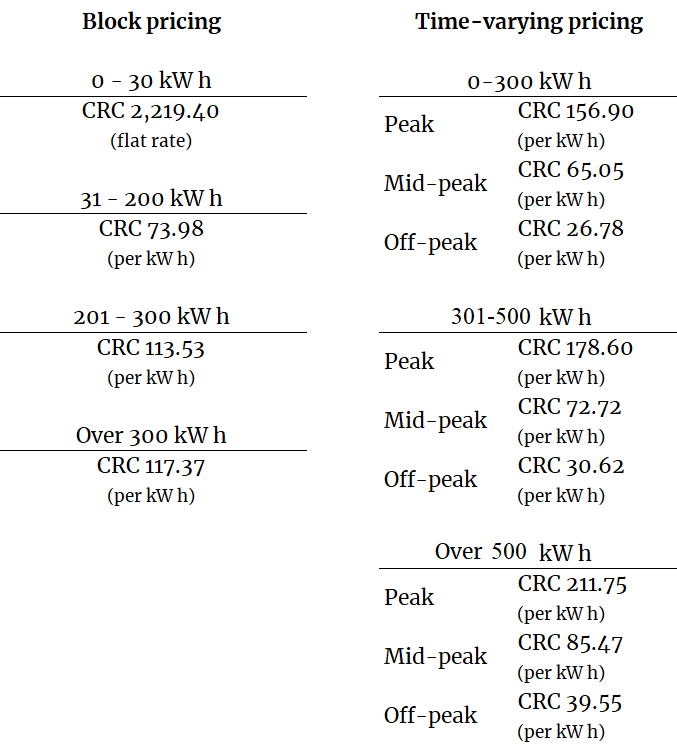
\includegraphics[width=1\textwidth]{./figures/table1.png}}
  \end{center}
\end{figure}

With the introduction of the time-varying pricing voluntary option, the CNFL offered a hybrid pricing schedule with characteristics of both block pricing and Time-of-Use pricing. Here, the CNFL divides consumers into three groups according to their monthly consumption: $0$ – $300$ kW h, $301$ – $500$ kW h, and over $500$ kW h. Each group pays the flat rate plus a rate per kW h that depends on the time of consumption. Just as before, prices are higher for groups with higher consumption. Within each group, the CNFL prices consumption depending on the time of usage: peak hours (10:00 to 12:30 and 17:30 to 20:00), mid-peak hours (06:01 to 10:00 and 12:30 to 17:30), and off-peak hours (20:00 to 06:00). These periods are defined based on historical aggregate consumption data. As an example, the right panel in Figure \ref{fig:table1} shows the rates for the TVP schedule during June 2019.

The program is voluntary, and the only requirement to join is for households to have a monthly consumption above $200$ kW h---which is similar than the average consumption in San José ($228$ kW h). While the CNFL promoted the program on their branches and social networks at the beginning early on (circa 2007), all efforts to promote the program ceased soon thereafter to avoid the cost of replacing the single-phase meter of new volunteers for a three-phase meter.\footnote{The financial health of the company changed for worse after the introduction of the TVP, for reasons unrelated to the TVP program.} This replacement is necessary to implement the TVP, because most consumers have a single-phase meter that only records the total electricity use since installation, but to price consumption at different times the CNFL needs to see consumption at different times. Because the CNFL stopped promoting the program early on, most of the people who signed up for the program did it at the beginning.

There is no data on why customers chose to join the program. Given that it was not promoted during the period of consumption that we can observe, we assume that most customers have never heard about the program and that those who joined after the CNFL stopped promoting the program found out either by word of mouth from a customer in the program, asking explicitly about the existence of such program to the CNFL, or perusing the CNFL’s website. Similarly, there is no data on why customers leave the program. Thus, unlike many papers that carefully model and explain how consumers self-select into TVP programs in other settings, we cannot explain selection. Instead, we focus on the still relevant local average treatment effect---for households that self-select, what is the effect of the TVP program on total consumption?

\section{Data and Methods}

We use monthly data of electricity consumption from 2011 to 2015 of all 444,352 CNFL residential electricity contracts.\footnote{After dropping data from 19 contracts of households that joined and left the program between 2011 and 2015.} Assuming each unique contract corresponds to one unique household, our unit of analysis is the household. This assumption is realistic and only leaves out a few special cases such as households with multiple homes. Unfortunately, we do not have data about any characteristics of the households.\footnote{The CNFL does not collect such data.} For months when a household is not in the TVP program, we only observe one value corresponding to their total monthly consumption. For months when a household is in the TVP program, we observe three values corresponding to total consumption during each of the three periods (i.e., peak, mid-peak, and off-peak hours).

There are two main issues with the data. First, the TVP program was introduced in 2007 and most of the households joined soon thereafter. Because we only observe consumption data starting in 2011, we are left with only $106$ households who joined the program between 2011 and 2015, as well as $555$ households who left the program in that period (See Figure \ref{fig:table2}). Thus, although we have monthly consumption data for about half a million households, only 7487 of them joined the program, and from these 7487, we only observe treatment status variation for 661 households. Second, because the program is voluntary and historical consumption over 200 kWh is required to join, households that joined the program might differ from the ones that did not join the program. We cannot address this self-selection into participation with our data. Instead, we identify groups of comparable households and obtain the local average treatment effect for each of these groups.

First, we group households according to their treatment status between 2011 and 2015: only out of the program ($O$), only in the program ($I$), joined ($J$), and left ($L$). All households in groups $I$, $J$, and $L$ were in the Time-Varying Pricing (TVP) program for at least one period, which implies both that they met the requirement of minimum historical consumption over 200 kW h and that they chose to join the program. Because households in these three groups are likely different from households in group $O$, comparing the consumption of households in groups $I$, $J$, or $L$ to the consumption of households in group $O$ to estimate the effect of the TVP program would likely lead to an estimate that reflects both the effect of the program and a self-selection bias.

\begin{figure}[ht]
  \caption{Number of households of each type}\label{fig:table2}
  \begin{center}
  {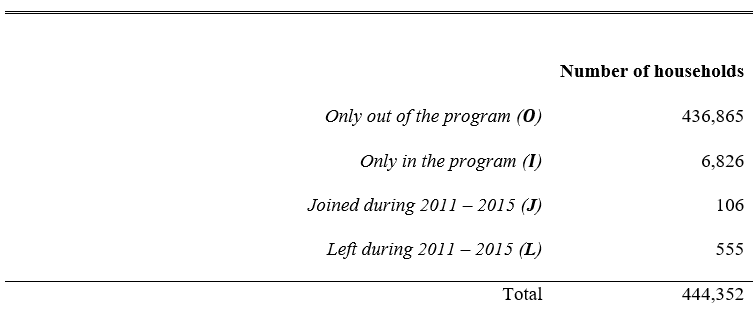
\includegraphics[width=1\textwidth]{./figures/table2.png}}
  \end{center}
\end{figure}

Indeed, as shown in Figure \ref{fig:one}, the average consumption of households that are only out of the program (group $O$) is about half of the average consumption of households in any of the other groups (see Figure \ref{fig:six} in the appendix for the difference between these groups over time). Because we do not have data to address the self-selection bias we would introduce by using households in group $O$ in our analyses, we drop from the analyses the data from all 436,865 households that were never in the TVP program. Therefore, we rely on comparisons between households in the remaining groups---$I$, $J$, and  $L$---to estimate the effect of the implementation of TVP on total consumption for households that self-selected into the program. For households from groups $J$ and $L$, the higher mean consumption when they were in the TVP program compared to when they were out of the program suggests that households increased their consumption due to the TVP schedule (Figure \ref{fig:one} and Figure \ref{fig:seven} in the appendix).

\begin{figure}[ht]
  \caption{Mean consumption by group and treatment status}\label{fig:one}
  \begin{center}
  {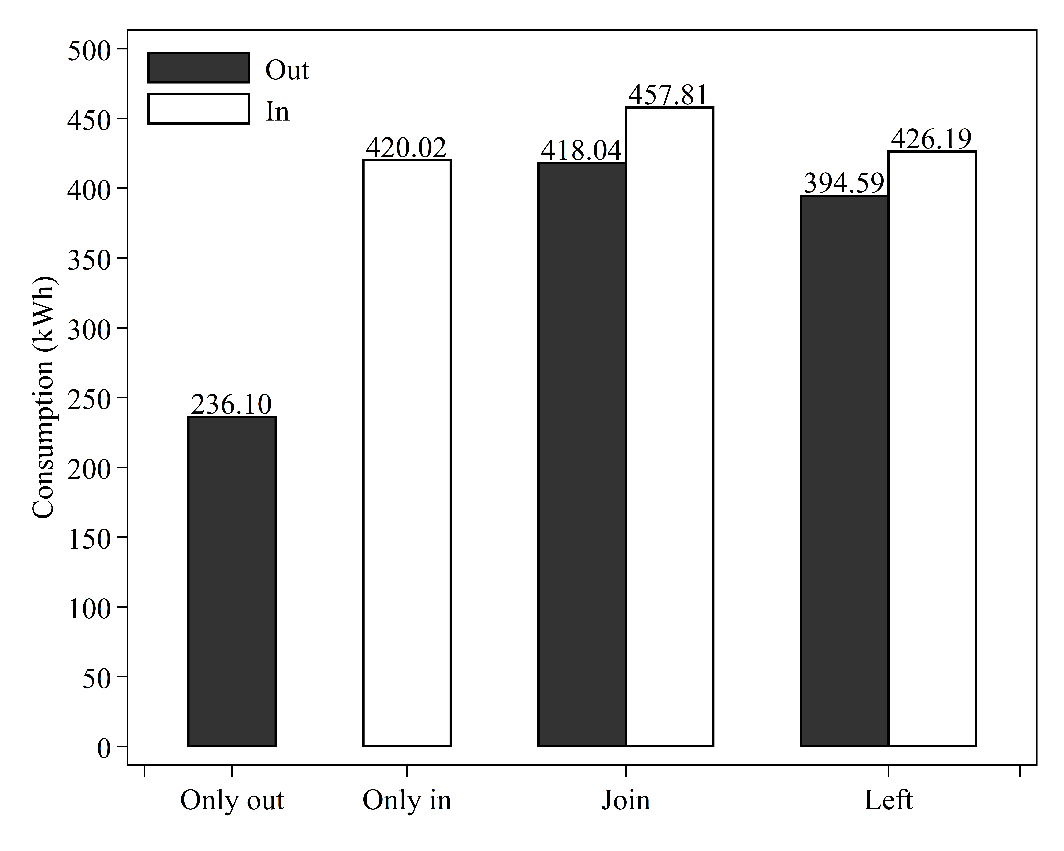
\includegraphics[width=1\textwidth]{./figures/image1.png}}
  \end{center}
\end{figure}

To estimate the effect of the time-varying pricing program (i.e., the treatment) on total consumption, we use a differences-in-differences (DD) research design and specify a two-way fixed effects differences-in-differences (TWFE) model. Explicitly, we use OLS to estimate

\begin{equation}
	y_{it} = \alpha_{i} + \lambda_{t} + \beta^{DD} D_{it} + \epsilon_{it}
\end{equation}

where $y_{it}$ is the electricity consumption of household $i$ in month $t$, $\alpha_{i}$ and $\lambda_{t}$ are household and time fixed effects, $D_{it}$ is a treatment dummy that is equal to 1 if household $i$ is in the program in month $t$ and 0 otherwise, and $\epsilon _{it}$ is the error term of the econometric model. The treatment effect is given by the coefficient $\beta^{DD}$. We present separate estimates for households that joined the program (group $J$) and households that left the program (group $L$). Thus, the impact is estimated by comparing the households before and after they joined the program, or before and after they left the program.

As opposed to the canonical differences-in-differences model with two periods and two groups, the interpretation of these estimates is not simply the difference between the difference from one period to another in the outcome variable of the treatment group and the difference from one period to another in the outcome variable of the control group. For example, consider a case with three periods. In the first period all households are not yet treated. In the second period, one group of households gets treated and the effect is estimated by comparing them to all the other households (i.e., same as in the canonical DD). In the third period, another group of households gets treated and the effect is estimated by comparing them to (1) the group of households that were already treated in the second period, and (2) the group of not-yet-treated households.

This three-period example shows that when multiple groups and periods are considered, the estimates of the treatment effect come from multiple comparisons between treatment and control groups, and these treatment and control groups vary in each period. More generally, \citet{goodman-baconDifferenceinDifferencesVariationTreatment2018} shows that the TWFE estimator when there is variation in when the treatment status changes is a weighted average of all possible two-group/two-period DD estimators in the data. For each of these $2 \times 2$ DD estimators, there is one control group whose treatment status does not change and one treatment group whose treatment status changes; and the weight is proportional to group sizes---size of the treatment and control groups---and the variance of the treatment variable. We use the exposition in \citet{goodman-baconDifferenceinDifferencesVariationTreatment2018} to explore and interpret our estimates.\footnote{We interpret our results following Goodman-Bacon (2018)'s work, but the literature on two-way fixed effects with heterogenous treatment effects is active; that is, recent advances are yet-to-be-published working papers. Relevant to this work, \citet{atheyDesignbasedAnalysisDifferenceInDifferences2018} show that, with staggered adoption, the standard DD estimator is unbiased. But the results rely on random assignment of the adoption date from a design perspective. \citet{dechaisemartinTwowayFixedEffects2020} explore the two-way fixed effects model with heterogeneous effects in general, and their special case of DD with staggered adoption is consistent with the exposition in \citet{goodman-baconDifferenceinDifferencesVariationTreatment2018}.}

Furthermore, we presume the treatment effect changes over time (i.e., it takes time to adjust behavior or make technological changes). This heterogeneity complicates the interpretation of the estimates from any TWFE DD model that relies on households that have already been treated acting as controls. To shed some light on the dynamics of the treatment effect to aid the interpretation of our estimates, we use an event-study specification.\footnote{\citet{sunEstimatingDynamicTreatment2020} show that the event-study specification is appropriate even with time-varying treatment effects if all cohort groups share the same dynamics, which we believe is a reasonable assumption for our context. } Explicitly, for the households that join (group $J$), we estimate:
\begin{equation}
	y_{it} = \alpha_{i} + \lambda_{t} + \sum_{\tau = 0}^{m} \delta_{- \tau}    D_{i,t - \tau} + \sum_{ \tau = 1}^{q} \gamma_{-\tau} D_{i,t + \tau} + \varepsilon_{it},
\end{equation}

% MUST CHECK THIS EQUATIOn

where $y_{it}$ is electricity consumption of household $i$ in month $t$, $\alpha_{i}$ and $\lambda_{t}$ are household and time fixed effects, the first summation term represents $\left( m-1 \right)$ leads or \enquote{before-treatment} effects and the second summation represents $q$ lags or \enquote{during-treatment} effects, and $\varepsilon_{it}$ is the error term of the econometric model. For the households that left (group $L$), we also estimate this equation but the leads represent the \enquote{during-treatment}  effects of the treatment and the lags represent the \enquote{after-treatment}  effects of treatment.

Finally, because the three-phase meters are only installed when a household is in the TVP program, we cannot observe consumption by time block for households that are not in the program.\footnote{\citet{jessoeUnderstandingRolePrice2014} overcame the lack of consumption data by period in their control group by using a complementary dataset of hourly consumption from a small sample of households in the utility. A similar dataset is not available for Costa Rica. \citet{allcottRethinkingRealtimeElectricity2011} randomized the TVP pricing over a population in which every household had a meter capable of keeping track of consumption by hour, therefore, he could observe consumption data by hour for both the control and experimental groups.} Without those data, it is not possible to estimate the effect of the TVP program on  peak consumption without very strong assumptions. In Appendix \ref{appendix:E}, we engage in a thought experiment to offer some suggestive evidence of the effect of TVP on peak consumption. That is, we use the fact that the time blocks of consumption (i.e., peak, mid-peak, and off-peak hours) were defined based on historical aggregate consumption data and assume that the consumption of the households in the program was consistent with the definition of the time blocks when they were not in the program. Although our results are only suggestive, they are in line with previous studies finding a decrease in electricity consumption during peak hours. In the results section we focus on the estimates of the effect of the TVP on total consumption.

\section{Results}

Table \ref{fig:table3} shows the (TWFE DD) estimates of the effect of Time-Varying Pricing (TVP) on total electricity consumption. All estimates are positive, with sizes ranging from 2\%  (6.8 kW h) to 16\% (67.9 kW h) of the average total consumption. However, these estimates are an average that reflects both the individual $2 \times 2$  DD estimators that can be constructed from the data and the weights of the TWFE estimator \citep{goodman-baconDifferenceinDifferencesVariationTreatment2018}. A detailed discussion follows.

\begin{figure}[ht]
  \caption{Effect of the TVP program on total consumption}\label{fig:table3}
  \begin{center}
  {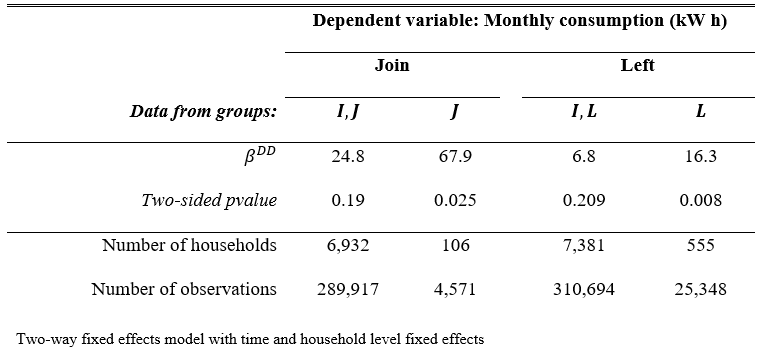
\includegraphics[width=1\textwidth]{./figures/table3.png}}
  \end{center}
\end{figure}


First, we consider the two TWFE estimates of the treatment effect for the households that joined the program between 2011 and 2015 (first two columns in Table 2). In the first column we present an estimate obtained using data both from households that were only in the program and households that joined the program (groups $I$ and $J$), and in the second column an estimate obtained using data from households that joined the program (group $J$).

In the TWFE estimate using only data from households in group $J$, there are only two types of $2 \times 2$ DDs: comparisons between \enquote{not-yet treated} households and \enquote{newly treated} households, and comparisons between \enquote{already treated} households and \enquote{newly treated}  households. Comparisons between \enquote{not-yet treated} households and \enquote{newly treated} households are akin to the comparison of pre and post periods in the canonical DD model. Comparisons between \enquote{already treated} households and \enquote{newly treated} households introduce a source of bias not present in the canonical DD model. Explicitly, when the treatment effect changes over time, the \enquote{already treated} households are no longer good controls and comparisons between them and \enquote{newly treated} households lead to biased DD estimates. In our case, there seems to be a declining trend of the treatment effect over time (see Figure \ref{fig:two}, and Figure \ref{fig:eight} and Figure \ref{fig:eleven} in the appendix). The bias reduces the DD estimate, because \enquote{already treated} households---whose treatment effect declines over time---are compared to \enquote{newly treated} households. In addition, the treatment status for most of the households changes within the first 4 periods of the observed data (see Figure \ref{fig:nine} in the appendix). The implication is that most of the  $2 \times 2$ DDs are estimated using \enquote{already-treated} households (with a declining treatment effect over time) as control. Further, the low variance of the treatment variable for the group cohorts in the first four periods leads to a lower weight for the DD estimate than what it is implied by their sample size (see Figure \ref{fig:ten} in the appendix).


Including data from households in group $I$---only in the program---changes both the DD terms and the weights of the terms. The DD terms change because the new group adds a new type of $2 \times 2$ DD: comparisons between \enquote{only in} and \enquote{newly treated} households. Thus, this case differs from the exposition in \citet{goodman-baconDifferenceinDifferencesVariationTreatment2018} in that he uses an \enquote{only out} instead of an \enquote{only in} group. The mechanics of the estimator remain the same---it is just a comparison between households for which treatment status changes and households for which treatment status does not change. However, by using \enquote{only in} instead of \enquote{only out} households, we again introduce a source of bias when treatment effects vary over time. What can be said about the bias in this case? Given a downward-sloping trend in the treatment effect, it is reasonable to assume that, on average, the treatment effect of the \enquote{only in} households is lower than the treatment effect of the \enquote{already treated} households. However, it is also reasonable to assume that households have had more time to adjust to the change in pricing schedule and the treatment effect is likely not changing over time as much as immediately after joining the program. As a result, either the treatment effect of the DDs from comparisons with \enquote{only in} households is lower or the negative bias from downward sloping treatment effect changes is stronger. In any case, the bias in the TWFE estimate is aggravated when including \enquote{only in} households. On the other hand, the weights of the $2 \times 2$  DD terms change because, while the variance of the treatment status remains the same, the absolute size of the subsample used in the DD and the relative share of control and treatment groups in each pair changes. As a result, the DDs comparing \enquote{only in} households---with a now lower treatment effect---to \enquote{newly treated} households get more weight and further reduce the TWFE estimate relative to the estimate obtained using only households from group $J$. Our estimates are likely to be a lower bound of the treatment effect of the program for the households that joined between 2011 and 2015.

Because it is not ideal to summarize a (potentially) time-varying treatment effect with a single coefficient, we try to capture the dynamics of the treatment effect with an event-study specification (see equation 2). The results using data of households that join (group $J$) are summarized in Figure \ref{fig:two}. The point estimates suggest no treatment effect before joining the program (the pvalue from an F-test is 0) and a positive but declining treatment effect after joining the program (the pvalue from an F-test is 0.52). However, we are unable to get precise estimates for most periods. For example, the 90\% confidence interval for the treatment effect 6 months before joining the TVP program ranges from about -250 kW h and 250 kW h. This lack of precision is because there are very few households treated 6 months (or later) after the start of the observed period (see Figure \ref{fig:nine} in the appendix).

\begin{figure}[ht]
  \caption{Event-study specification for households that joined the program}\label{fig:two}
  \begin{center}
  {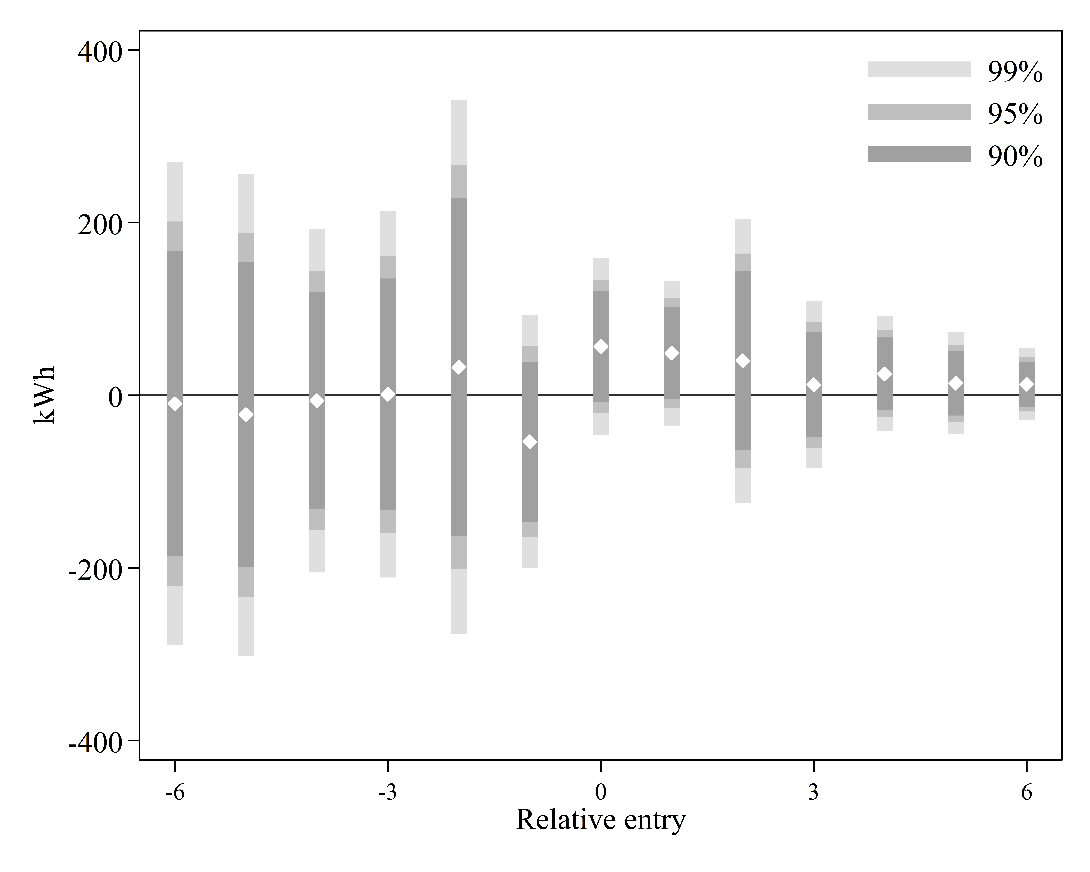
\includegraphics[width=1\textwidth]{./figures/image2.png}}
  \end{center}
\end{figure}

Let us return to now to the TWFE estimates for the households that left the program between 2011 and 2015 (Figure \ref{fig:table3}, last two columns). In column 3 we present an estimate obtained using data both from households that were only in the program and households that left the program (groups $I$ and  $L$), and in column 4 an estimate obtained using only data from households that left the program (group $L$). Relative to when households joined the program, the analysis for households that left is flipped. Instead of estimating the treatment effect by using the change in consumption when households join, we estimate the treatment effect by using the change in consumption when households leave. Alternatively, the interpretation is that the change in treatment status goes from \enquote{join the program} to \enquote{leave the program}. That is, we say that when a household changes its treatment status---leaves the program---it becomes \enquote{newly untreated}.

In the TWFE estimate using only data from households in group $L$, there are only two types of $2 \times 2$  DDs: comparisons between \enquote{not-yet untreated} households and the \enquote{newly untreated} households, and comparisons between \enquote{already untreated} households and \enquote{newly untreated} households. Unlike the case with data from group $J$---in which the time-varying treatment effect affects households’ consumption \emph{after} they change their treatment status to treated---here the change in treatment status to untreated implies that households’ consumption is affected by the time-varying treatment effect \emph{before} their change in treatment status. Therefore, we get the opposite result from the case when households join the program: the second type of DDs is akin to the canonical DD model with two periods and the first type of DDs introduces a source of bias when treatment effects vary over time.

From the previous case, it seems that the treatment effect declines over time for households that joined (see Figure \ref{fig:two}, and Figure \ref{fig:eight} and Figure \ref{fig:eleven} in the appendix). We infer that households \enquote{only in} the program are likely have a lower treatment effect or that changes---if any---over time are lower than when households recently joined the program. And data from households that left suggest that the treatment effect increases over time (see Figure \ref{fig:three}, and Figure \ref{fig:twelve} and \ref{fig:fifteen} in the appendix). Therefore, the estimate with only data from group $L$ is likely to have a positive bias that inflates the treatment effect. While still reflecting the positive bias from the upward-sloping time-varying treatment effect, including data from group $I$ is likely to reduce the effect in two ways. First, the $2 \times 2 $ DD estimators of comparisons with the \enquote{always treated} are likely to be, on average, lower than the average  $2 \times 2$  DD estimator from the TWFE using only households from group $L$. Second, while the variance of the treatment status remains the same, with the new data, the absolute size of the subsample used in the DDs and the relative share of control and treatment groups in each pair changes. The implication is that the weight of the DDs biased by the upward-sloping time-varying treatment effect is lower than before. Because there are opposite forces at play, the interpretation of the bias in the estimates in this case is ambiguous. The TWFE estimate using only data from group $L$ is likely higher than the true effect, but we cannot infer the net result of the opposing effects at play when including the data from group $I$.

Of course, the upward-sloping time-varying treatment effect for households that left might be the reason households left the program (see Figure \ref{fig:three} and Figure \ref{fig:twelve} in the appendix). In fact, households in group $L$ have the highest hourly consumption during peak hours relative to the hourly consumption during mid-peak hours of all groups that self-selected into the program (see Figure \ref{fig:seventeen} in the appendix). They also seem to have the highest hourly consumption during peak hours (see Figure \ref{fig:eightteen} in the appendix), and yet have the lowest total consumption of all groups (see Figure \ref{fig:sixteen} in the appendix). In the absence of direct information from the households that left, the discussion remains largely speculative, but it seems that these households are less able to adjust their consumption during the day to exploit the benefits of the TVP pricing and, given their lower total consumption, pay a higher price as a share of the total bill for their lack of flexibility. Still, one can redefine the treatment as \enquote{leaving the program} and, through the lens of a Roy model of selection on gains \citep{heckmanChapter70Econometric2007}, interpret the results as an upper bound of the average effect on total consumption of changing the pricing from TVP to a non-TVP schedule.

% add discussion of mistakes in forecasting potential gains from entering the program. Perhaps in the paragraph below

Given the previous discussion, the appropriateness of combining data from groups  $I$ and $L$ to get the TWFE estimate is not undisputable. If households that left the program are different than households that were always in the program, combining them would lead to an estimate biased due to self-selection into leaving the program.

Again, we try to capture the dynamics of the treatment effect with an event study specification, but this time using data from group $L$. The results are summarized in Figure \ref{fig:three}. The point estimates suggest a positive treatment effect when households are in the program (the pvalue from an F-test is 0) and no treatment effect when households are not in the program (the pvalue from an F-test is 0.15). As opposed to the case using data from group  $J$, here we obtain more precise estimates because there is a similar number of households leaving the program each month (see Figures \ref{fig:thirteen} and \ref{fig:fourteen} in the appendix). In other words, the sizes of the control and treatment groups are more equal.

\begin{figure}[ht]
  \caption{Event-study specification for households that left the program}\label{fig:three}
  \begin{center}
  {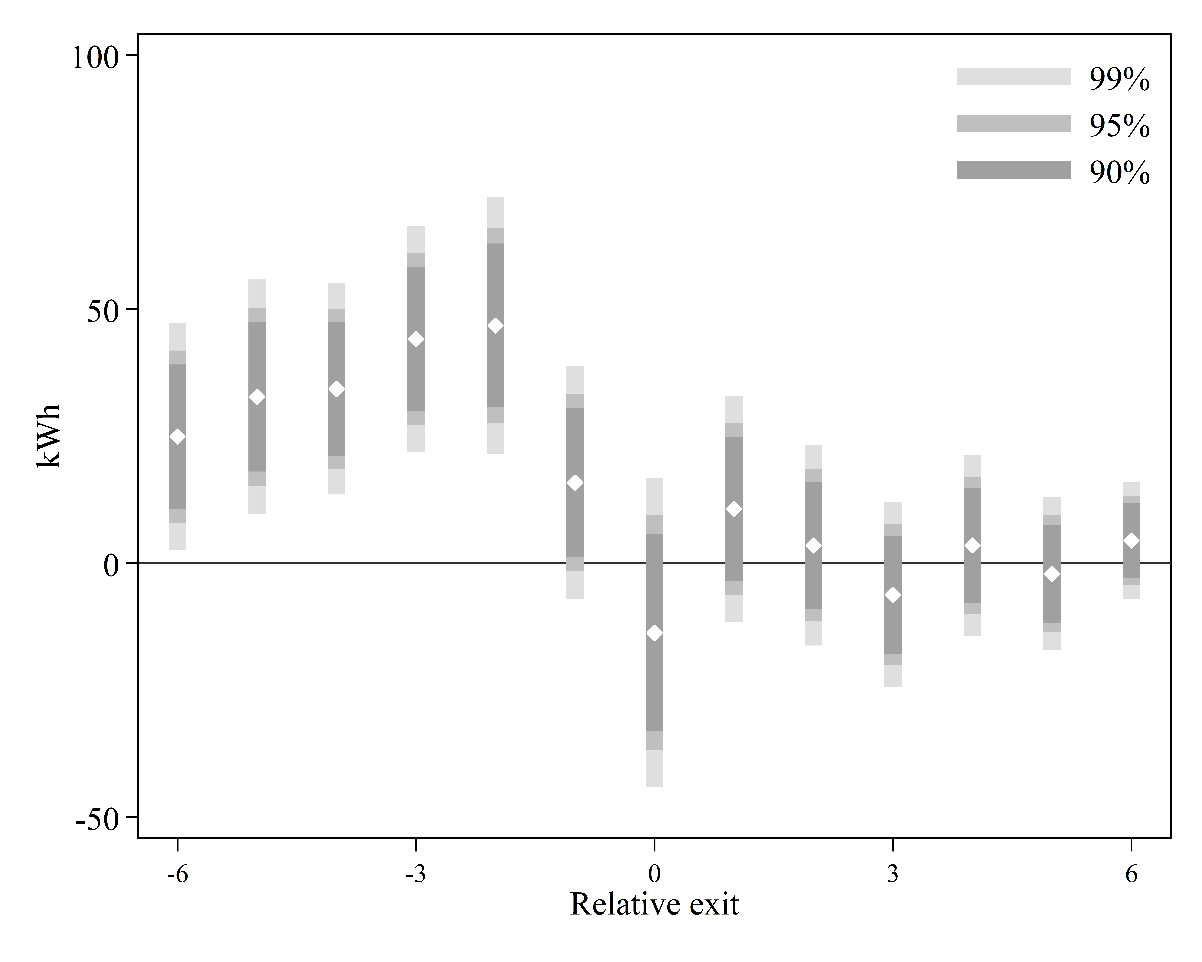
\includegraphics[width=1\textwidth]{./figures/image3.png}}
  \end{center}
\end{figure}

In summary, given the data constraints, we have not provided unbiased estimates of the effect of a time-varying pricing program on total consumption. However, we argue that we have provided evidence suggesting that, contrary to findings from previous research, the effect of the implementation of TVP on total consumption might not be negative. Instead, it seems that when there is little to no room for technological change and behavioral change to drive changes in consumption, households that self-select into the TVP program may increase their total consumption.

\section{Reconciling seemingly conflicted results}

While previous research finds that households decrease total electricity consumption in response to Time-Varying Pricing (TVP), we find the opposite. How to reconcile this seemingly mixed evidence? First, consider a world with no technological changes and a two-period TVP program (i.e., peak and off-peak). A household in this program faces two separate demand curves, one during peak hours and one during off-peak hours.\footnote{The price during peak hours is higher than the constant price before the TVP, and the price during the off-peak hours is lower than the constant price before the TVP.} Without substitution over time (i.e., cooking late at night instead of during the evening), consumption decreases during peak hours and increases during off-peak hours (Figure \ref{fig:four}, top panel). With substitution over time, the household’s demand curve during peak hours shifts to the left by the amount of consumption that is possible to substitute over time, with a corresponding shift to the right in the demand curve during off-peak hours. Critically, every kW h \enquote{transferred} from peak hours to off-peak hours is transformed into more than 1 kW h because of the lower price.\footnote{Here we discuss only the consequences of a change in price. However, there are alternative mechanisms that could lead to changes in the amount of electricity consumed when activities that use electricity are shifted from peak hours to off peak hours. For example, in response to the TVP pricing, one could take a bath late at night instead of in the morning. Without the need to leave home to work, the bath might be longer (resulting in more electricity use) simply because now there is more time to enjoy it (beyond the increased use that can be explained by the lower price per kW h). We thank Jo Albers for bringing up the potential role of mechanisms beyond the response to lower prices.} In both cases, the effect of the TVP on total consumption is simply the net effect $ \left( q_{0}^{peak}-q_{1}^{peak} \right) + \left( q_{1}^{off}-q_{0}^{off} \right) $.

\begin{figure}[ht]
  \caption{Behavioral changes in response to TVP}\label{fig:four}
  \begin{center}
  {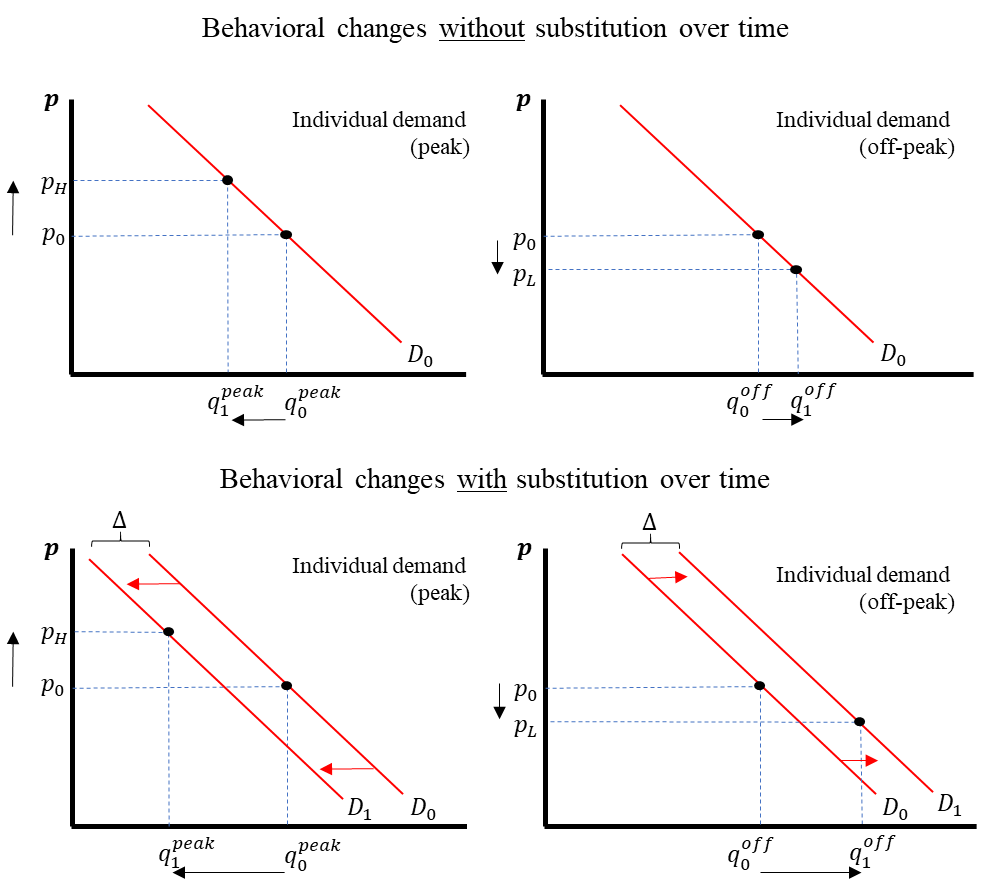
\includegraphics[width=1\textwidth]{./figures/image4.png}}
  \end{center}
\end{figure}

Second, assume that households respond to an average price\footnote{ \citet{itoConsumersRespondMarginal2014}, for example, show that households do not seem to respond to marginal electricity prices. Instead, they respond to some average price.}
\begin{equation}
	p^{TVP} = p_{H} w^{peak} + p_{L} w^{off},
\end{equation}
where $p_{H}$ is the price of the TVP during peak hours, $p_{L}$ is the price of the TVP during off-peak hours, and $w^{peak}$ and $w^{off}$ are weights describing the relative amount of consumption of the household in each of the two periods, with $w^{peak} + w^{off} = 1$. By revealed preference (households self-selected into the program), we have that $p^{TVP} < p_{o}$, where $p_{0}$ is the constant price of electricity before the implementation of the TVP program.\footnote{We can explain the existence of people sophisticated enough to choose a TVP schedule but not sophisticated enough to make day-to-day electricity consumption choices based on marginal prices in at least two ways. First, they might be choosing the TVP under the influence of some optimism bias. Second, they might be rationally inattentive; it is worth to spend the time thinking about which pricing schedule to choose, but it might not be worth to spent too much time thinking about everyday electricity consumption choices such as turning off a lightbulb. We thank Sarah Jacobson for raising this issue.}

Third, a household responding to $p^{TVP}$ with only behavioral changes increases total consumption simply because $p^{TVP} <p_{o}$ (Figure \ref{fig:five}, left panel). Instead, a household responding to $p^{TVP}$ with both technological and behavioral changes may either reduce or increase total consumption (Figure \ref{fig:five}, right panel). Here, the technological changes shift the demand curve to the left (i.e., because of a new fridge that uses less electricity all day). Along the new demand curve ($D_{1}$), households increase consumption because $p^{TVP} < p_{o}$ . Whether the net effect is an increase or decrease depends on the relative size of the effect coming from technological changes and behavioral changes. We reconcile the seemingly mixed evidence by noting that our results come from a setting with almost no room for technological changes (Figure \ref{fig:five}, left panel), and previous results come from a setting in which there is plenty room for technological changes (Figure \ref{fig:five}, right panel).

\begin{figure}[ht]
  \caption{Only behavioral changes vs behavioral and technological changes}\label{fig:five}
  \begin{center}
  {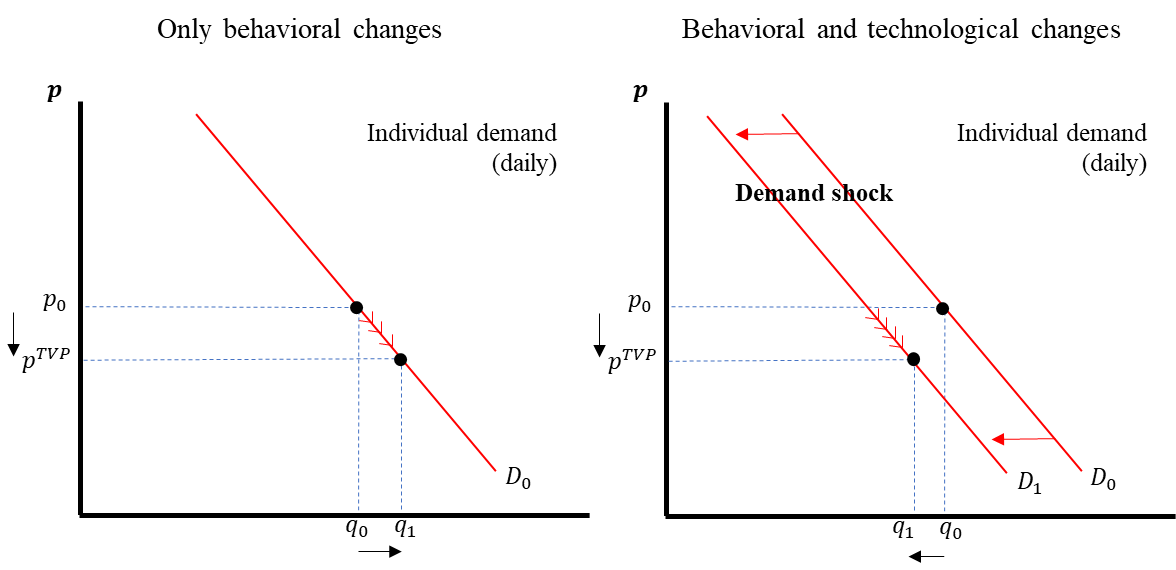
\includegraphics[width=1\textwidth]{./figures/image5.png}}
  \end{center}
\end{figure}

\section{Conclusion}

Empirical research has shown that using time-varying pricing (TVP) helps to solve the allocative inefficiency in the residential electricity sector \citep{allcottRethinkingRealtimeElectricity2011,wolakResidentialCustomersRespond2011,jessoeUnderstandingRolePrice2014}. Explicitly, researchers consistently find that TVP schedules reduce both total consumption and consumption during peak hours. However, none of these studies have explicitly addressed the separate effects of technological and behavioral changes in consumption when a TVP schedule is implemented.

To partially isolate the effect on total consumption of behavioral changes in response to TVP, we study a voluntary program that introduced a TVP schedule to households in San José, the capital of Costa Rica. We chose San José because it has a mild climate and very few households use heating or cooling devices. With little room for technological changes (relative to a rich country), consumption changes are largely driven by behavioral changes. Contrary to previous research, we find that TVP may increase total electricity consumption. However, we argue that this seemingly conflicting result should not be considered contradictory. Instead, we show how the difference between our result and previous findings is explained by the differences in the context of the studies.

Despite variation in the timing of the treatment and a potential time-varying treatment effect, we are able to present suggestive evidence that households may increase consumption in response to TVP. To do so, we exploit recent econometric developments on the understanding of the two-way fixed effects differences-in-differences estimator \citep{goodman-baconDifferenceinDifferencesVariationTreatment2018} along with event-study specifications to interpret our results. Given data limitations and the general issues with capturing a potentially dynamic effect with one coefficient, we believe that the recent econometric developments expand the scope of what is possible to learn using a differences-in-differences research design.

We also emphasize the need for better data to study time-varying prices in alternative contexts. While in this paper we work with what was reasonable to collect, we had to rely on somewhat strong assumptions to provide suggestive evidence of the effects of implementing a TVP schedule (e.g., our discussion of biases in the TWFE DD estimates). In contrast, most of the previous studies have relied on rich data from large randomized control trials (Faruqui $\&$  Sergici, 2010; Badtke-Berkow et al, 2015). Because the incentives of the electric utilities are aligned with the potential efficiency gains of TVP pricing, researchers and utilities could work together to generate the data required for a comprehensive analysis of TVP in alternative contexts. There are still open questions that can only be answered with better data. For example, \citep{itoConsumersRespondMarginal2014} shows that households do not respond to marginal prices of electricity; instead, they respond to \emph{some} average price. In our context, we find suggestive evidence along the same lines (see Figure \ref{fig:nineteen} in the appendix), but little can be said about the average prices to which households respond.


% HERE!

Finally, our research could help policy makers better anticipate the likely effects of implementing time-varying prices in different contexts. For example, when implementing a TVP schedule in a context with low usage of heating and cooling devices, policy makers would know not to expect reductions in consumption during peak hours as large as those found by previous research. Further, our finding of an increase in total electricity consumption due to the TVP schedule challenges previous research on the short-run and long-run expected outcomes of TVP (Borenstein, 2005). In addition, we are not aware of any previous study on the effect of TVP in a non-rich country. Our hope is that policy makers in contexts closer to ours than to a rich country will be able to use this study to motivate policy making using empirical evidence relevant to their own context. Specifically, our results serve as a cautionary piece of evidence for policy makers interested in reducing consumption during peak hours with TVP---the goal can potentially be achieved, but the cost is increased total consumption. Therefore, policy makers should weight both policy targets carefully before opting for TVP.

\clearpage

% REFERENCES -------------------------------------------------------------------

\bibliography{CNFL}

\clearpage

% ACKNOWLEDGEMENTS -------------------------------------------------------------

\section*{Acknowledgements}

Our work was improved thanks to useful comments by David Aadland, Jo Albers, Hunt Allcott, Sara Capitán, Benjamin Gilbert, Sarah Jacobson, Marc Jeuland, Esteban Méndez-Chacón, Alexandre Skiba, Linda Thunström, Klaas van 't Veld, and Donald Waldman.

Our work also reflects improvements in response to comments by participants at the Third Annual Meeting of the Sustainable Energy Transitions Initiative, the 2018 Colorado State University and University of Wyoming joint Graduate Student Symposium, the 20th Colorado University at Boulder Environmental and Resource Economics Workshop, and the 2020 Online Summer Workshop in Environment, Energy, and Transportation (Economics).

Finally, we thank the \emph{Compañia Nacional de Fuerza y Luz} for sharing the data used in this research, and the economic support from the Swedish Agency for International Development Cooperation (SIDA) through the Environment for Development (EfD) initiative.


\clearpage

% APPENDICES -------------------------------------------------------------------
% \begin{appendices}
%
%   \startcontents[sections]
%   \printcontents[sections]{l}{1}{\setcounter{tocdepth}{1}}
%
%   \clearpage
%
% \section{Conceptual framework}
%
%   \label{appendix:appendix_conceptualFramework}
%
%   \input{parts/appendix_conceptualFramework.tex}
%
%   % add link back to document
%
% \clearpage
%
% \end{appendices}


\end{document}

% END OF FILE ------------------------------------------------------------------
% ------------------------------------------------------------------------------
